\documentclass{article}

\usepackage{graphicx}
\usepackage{tikz}
\usepackage{tikzsymbols}
\usetikzlibrary{calc,patterns,shapes.geometric}
\pagestyle{empty}
\usepackage[margin=0pt]{geometry}
\geometry{papersize={14in,12in}}

\def\centerarc[#1](#2)(#3:#4:#5){\draw[#1] ($(#2)+({#5*cos(#3)},{#5*sin(#3)})$) arc (#3:#4:#5);}

\begin{document}
	\begin{figure}
		\centering
		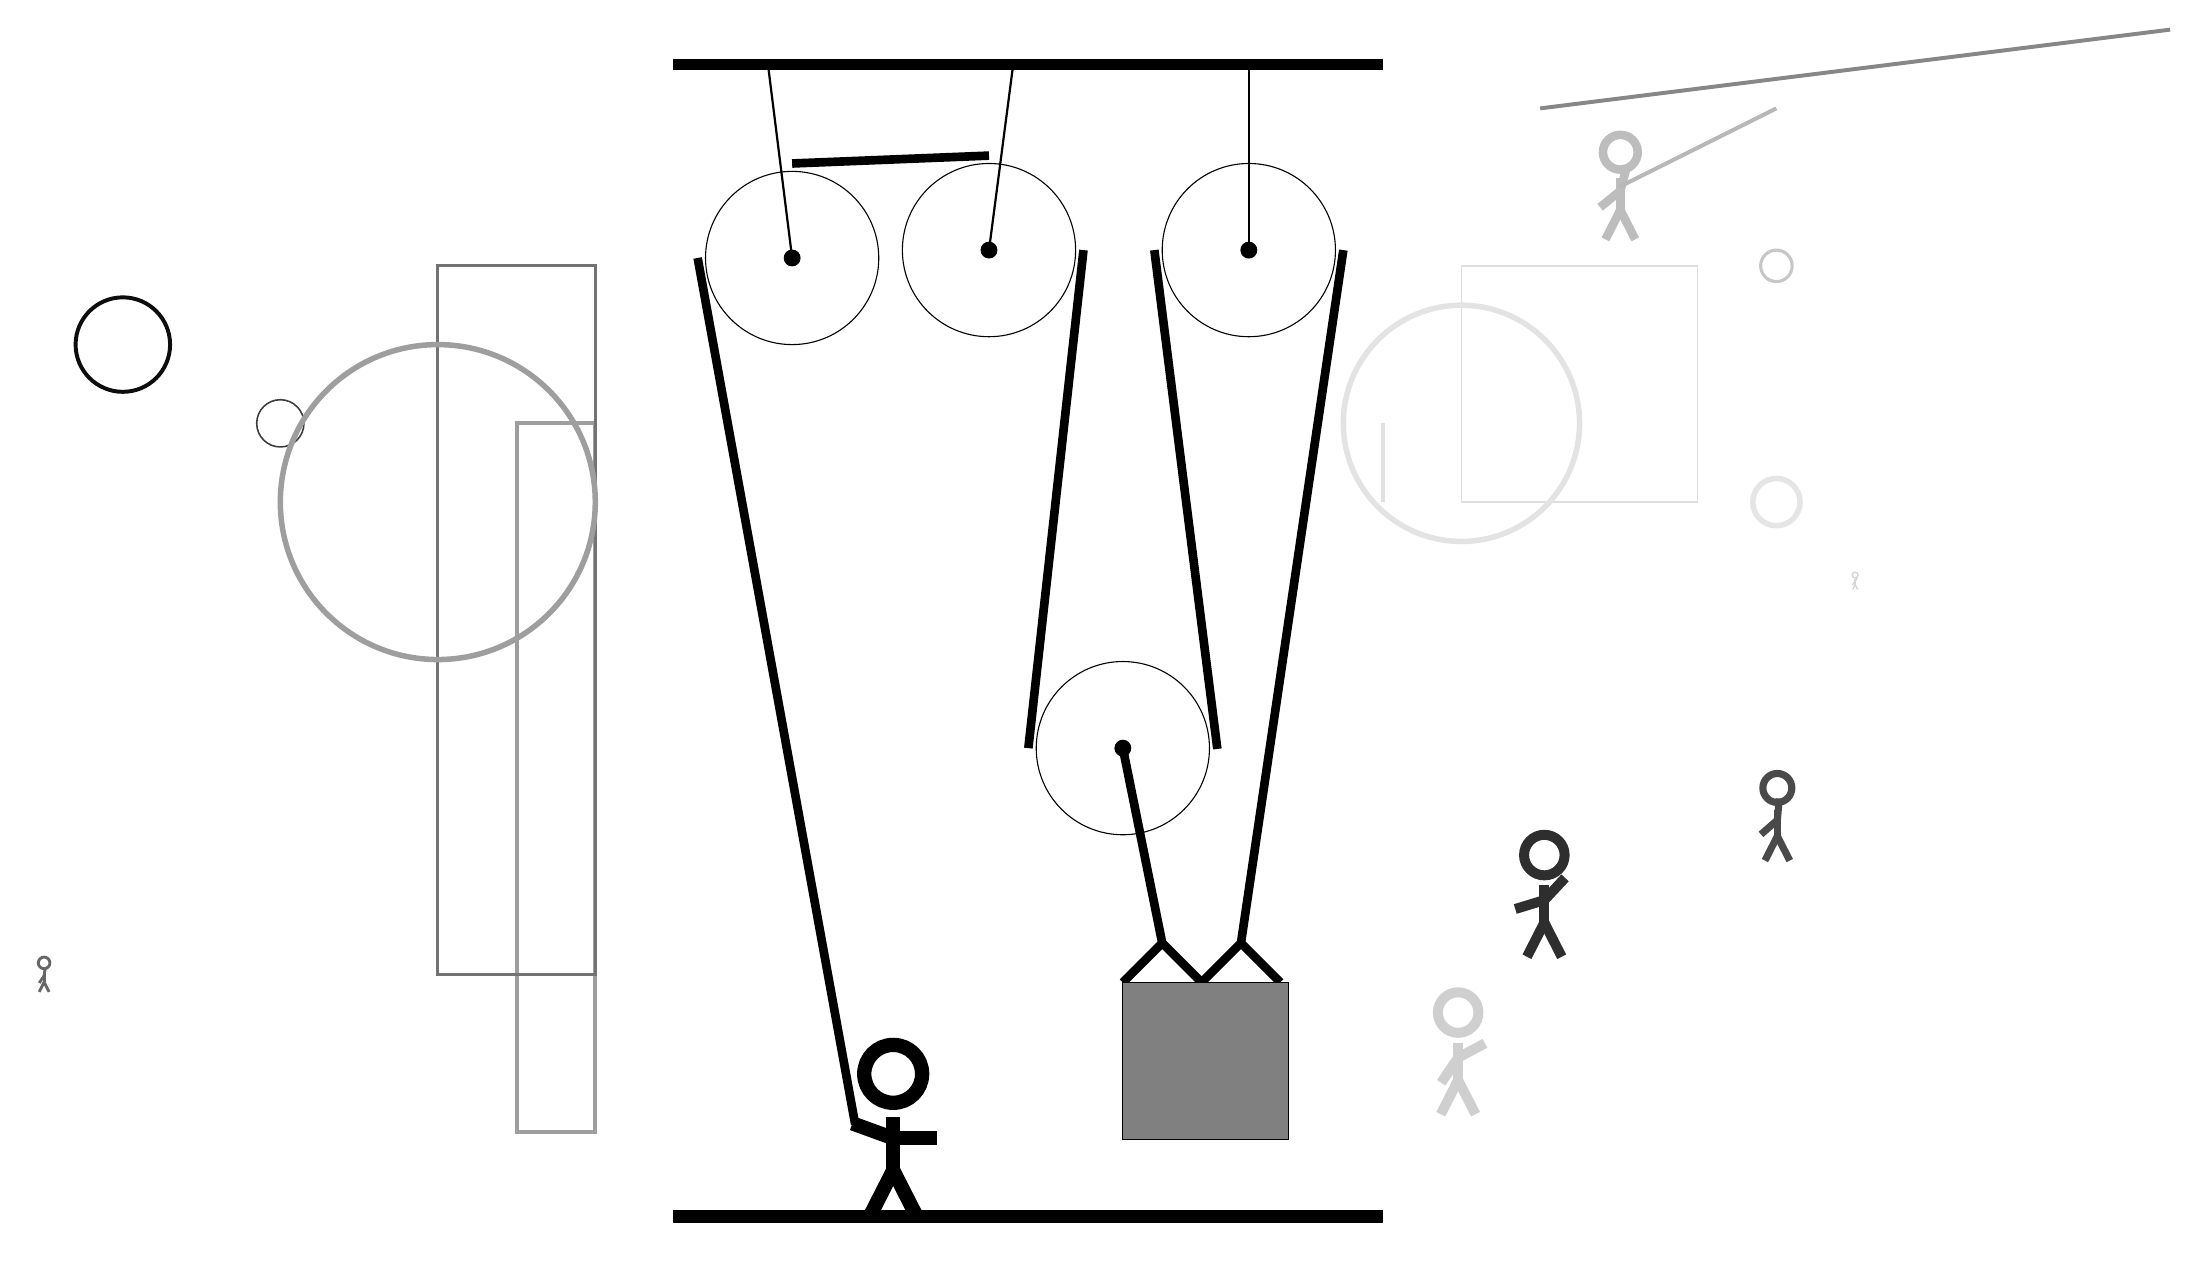
\begin{tikzpicture}
			%%%%% START %%%%%
			
			\draw[fill=black] (-3, 11.5) rectangle (6, 11.625);
			
			\draw (1, 9.2) circle (1.1);
			\draw[fill=black] (1, 9.2) circle (0.1);
			\draw[thick] (1, 9.2) -- (1.3, 11.5);
			
			\draw (4.3, 9.2) circle (1.1);
			\draw[fill=black] (4.3, 9.2) circle (0.1);
			\draw[thick] (4.3, 9.2) -- (4.3, 11.5);
			
			\draw (2.7, 2.875) circle (1.1);
			\draw[fill=black] (2.7, 2.875) circle (0.1);
			
			\draw[line width=1.1mm]  (2.7, -0.1) -- (3.2, 0.4) -- (3.7, -0.1) -- (4.2, 0.4) -- (4.7, -0.1);
			\draw[fill=black!50] (2.7, -0.1) rectangle (4.8, -2.1);
			
			\draw (-1.5, 9.1) circle (1.1);
			\draw[fill=black] (-1.5, 9.1) circle (0.1);
			\draw[thick] (-1.5, 9.1) -- (-1.8, 11.5);
			
			\draw [line width=0.4mm, color=black!22](11, 9) circle (0.2);
			
			\draw [line width=0.5mm, color=black!95](-10, 8) circle (0.6);
			\node[line width=0.3mm, color=black!16] at (12, 5) {\Strichmaxerl[1][51][60]};
			\draw [line width=0.7mm, color=black!10](11, 6) circle (0.3);
			\draw[line width=0.3mm, color=black!30] (-5, 1) rectangle (-5, 3);
			\draw[line width=0.5mm, color=black!38] (-5, -2) rectangle (-4, 7);
			\draw [line width=0.2mm, color=black!76](-8, 7) circle (0.3);
			\draw[line width=0.4mm, color=black!55] (-4, 9) rectangle (-6, 0);
			\node[line width=0.5mm, color=black!26] at (9, 10) {\Strichmaxerl[6][39][75]};
			\node[line width=0.5mm, color=black!71] at (11, 2) {\Strichmaxerl[5][41][85]};
			\draw [line width=0.6mm, color=black!78](11, 8) circle (0.0);
			
			\draw[line width=0.2mm, color=black!13] (7, 9) rectangle (10, 6);
			\draw [line width=0.7mm, color=black!11](7, 7) circle (1.5);
			
			\node[line width=0.4mm, color=black!60] at (-11, 0) {\Strichmaxerl[2][56][82]};
			\draw[line width=0.5mm, color=black!12](6, 7) -- (6, 6);
			\draw[line width=0.5mm, color=black!28](11, 11) -- (9, 10);
			
			\node[line width=0.6mm, color=black!19] at (7, -1) {\Strichmaxerl[7][56][28]};
			
			\draw[line width=0.5mm, color=black!47](8, 11) -- (16, 12);
			\draw [line width=0.7mm, color=black!38](-6, 6) circle (2.0);
			
			\node[line width=0.2mm, color=black!82] at (8, 1) {\Strichmaxerl[7][17][47]};
			
			\draw[line width=1.1mm](-0.7, -1.9) --  (-2.7, 9.1);
			\centerarc[line width=1.1mm](-1.5, 9.1)(90:180:1.2000000000000002);
			\draw[line width=1.1mm](-1.5, 10.3) -- (1, 10.4);
			\centerarc[line width=1.1mm](1, 9.2)(0:90:1.2000000000000002);
			\draw[line width=1.1mm](2.2, 9.2) -- (1.5, 2.875);
			\centerarc[line width=1.1mm](2.7, 2.875)(180:370:1.2000000000000002);
			\draw[line width=1.1mm] (3.9, 2.865) -- (3.1, 9.2);
			\centerarc[line width=1.1mm](4.3, 9.2)(0:180:1.2000000000000002);
			\draw[line width=1.1mm](4.2, 0.4) -- (5.5, 9.2);
			\draw[line width=1.1mm] (3.2, 0.4) -- (2.7, 2.875);
			
			\node at (-0.2, -2) {\Strichmaxerl[10][-20][0]};
			
			\draw[fill=black] (-3, -3) rectangle (6, -3.15);
			
			%%%%% END %%%%%
		\end{tikzpicture}
	\end{figure}	
\end{document}